% ============================================================================
% Chapitre 4 : R\'eseaux de Neurones Convolutifs (CNN)
% ============================================================================
\chapter{R\'eseaux de Neurones Convolutifs (CNN)}
\label{ch:cnn}

\noindent\textit{Ce chapitre pr\'esente les r\'eseaux de neurones convolutifs, une famille
d'architectures sp\'ecialis\'ees pour le traitement de donn\'ees structur\'ees
spatialement. Nous d\'erivons les op\'erations fondamentales, \'etudions les
architectures historiques et modernes, et d\'emontrons math\'ematiquement les
propri\'et\'es qui font le succ\`es des connexions r\'esiduelles.}\medskip

% ----------------------------------------------------------------------------
\section{Motivations}
\label{sec:cnn-motivations}
\index{CNN!motivations}

Les r\'eseaux enti\`erement connect\'es pr\'esentent trois limitations
majeures pour le traitement des images :

\begin{definition}[Principes inductifs des CNN]
Les CNN exploitent trois principes :
\begin{enumerate}
  \item \textbf{Localit\'e} : les caract\'eristiques visuelles sont d\'efinies
    par des motifs locaux (ar\^etes, textures).
    \index{localit\'e}
  \item \textbf{Invariance par translation} : un motif visuel peut appara\^itre
    n'importe o\`u dans l'image.
    \index{invariance par translation}
  \item \textbf{Partage des param\`etres} : le m\^eme filtre est appliqu\'e
    \`a toutes les positions spatiales, r\'eduisant drastiquement le nombre de
    param\`etres.
    \index{partage des param\`etres}
\end{enumerate}
\end{definition}

\begin{remarque}[R\'eduction des param\`etres]
Pour une image $224 \times 224 \times 3$, une couche enti\`erement connect\'ee
vers 1000 neurones n\'ecessite $224 \times 224 \times 3 \times 1000 \approx 150$M
param\`etres. Une couche convolutive avec 64 filtres $3 \times 3$ n'en
requiert que $3 \times 3 \times 3 \times 64 = 1\,728$ param\`etres.
\end{remarque}

% ----------------------------------------------------------------------------
\section{Op\'eration de convolution}
\label{sec:convolution}
\index{convolution}

\subsection{Convolution discr\`ete 2D}

Pour une entr\'ee $\mathbf{X} \in \R^{H \times W}$ et un noyau
$\mathbf{K} \in \R^{k_H \times k_W}$, la convolution discr\`ete
(plus pr\'ecis\'ement la corr\'elation crois\'ee) est :

\begin{formules}[title=\textbf{Convolution 2D}]
\begin{equation}
(\mathbf{X} * \mathbf{K})[i, j] = \sum_{m=0}^{k_H - 1} \sum_{n=0}^{k_W - 1}
  \mathbf{X}[i + m, j + n] \cdot \mathbf{K}[m, n]
\label{eq:conv2d}
\end{equation}
\end{formules}

\subsection{Taille de sortie}

\begin{theoreme}[Formule de la taille de sortie]
Pour une entr\'ee de taille $H \times W$, un noyau $k \times k$, un padding
$p$ et un stride $s$, la taille de sortie est :
\begin{equation}
H_{\text{out}} = \left\lfloor \frac{H - k + 2p}{s} \right\rfloor + 1, \qquad
W_{\text{out}} = \left\lfloor \frac{W - k + 2p}{s} \right\rfloor + 1
\label{eq:conv-output-size}
\end{equation}
\end{theoreme}

\begin{exemple}[Calcul de taille]
Entr\'ee $32 \times 32$, noyau $5 \times 5$, padding $p = 2$, stride $s = 1$ :
\[
H_{\text{out}} = \left\lfloor \frac{32 - 5 + 4}{1} \right\rfloor + 1 = 32
\]
Le padding $p = \lfloor k/2 \rfloor$ pr\'eserve la taille spatiale
(<<~same padding~>>).
\end{exemple}

\subsection{Convolution multi-canaux}

Pour $C_{\text{in}}$ canaux d'entr\'ee et $C_{\text{out}}$ filtres :
\begin{equation}
\mathbf{Y}[c_{\text{out}}, i, j] = b_{c_{\text{out}}} +
\sum_{c_{\text{in}}=0}^{C_{\text{in}}-1}
\sum_{m=0}^{k_H-1} \sum_{n=0}^{k_W-1}
\mathbf{X}[c_{\text{in}}, i{+}m, j{+}n] \cdot
\mathbf{K}[c_{\text{out}}, c_{\text{in}}, m, n]
\end{equation}

Nombre total de param\`etres : $C_{\text{out}} \times (C_{\text{in}} \times k_H \times k_W + 1)$.

\subsection{Diagramme de l'op\'eration de convolution}

\begin{center}
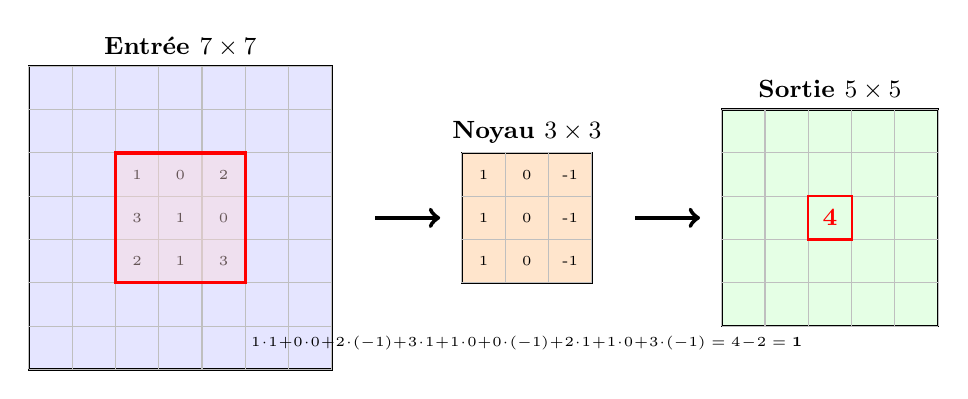
\begin{tikzpicture}[scale=0.55]
  % Entr'ee
  \draw[fill=blue!10, thick] (0,0) rectangle (7,7);
  \node[above, font=\small\bfseries] at (3.5, 7) {Entr\'ee $7 \times 7$};

  % Grille
  \foreach \i in {0,...,7} {
    \draw[gray!50] (\i, 0) -- (\i, 7);
    \draw[gray!50] (0, \i) -- (7, \i);
  }

  % Valeurs dans l'entr'ee (sous-r'egion)
  \foreach \i/\j/\v in {
    2/4/1, 3/4/0, 4/4/2,
    2/3/3, 3/3/1, 4/3/0,
    2/2/2, 3/2/1, 4/2/3} {
    \node[font=\tiny] at (\i+0.5, \j+0.5) {\v};
  }

  % Surbrillance du r'eceptive field
  \draw[red, very thick, fill=red!15, fill opacity=0.4] (2,2) rectangle (5,5);

  % Fl`eche
  \draw[->, ultra thick] (8, 3.5) -- (9.5, 3.5);

  % Noyau
  \draw[fill=orange!20, thick] (10, 2) rectangle (13, 5);
  \foreach \i in {10,...,13} {
    \draw[gray!50] (\i, 2) -- (\i, 5);
    \draw[gray!50] (10, \i-8) -- (13, \i-8);
  }
  \foreach \i/\j/\v in {
    10/4/1, 11/4/0, 12/4/-1,
    10/3/1, 11/3/0, 12/3/-1,
    10/2/1, 11/2/0, 12/2/-1} {
    \node[font=\tiny] at (\i+0.5, \j+0.5) {\v};
  }
  \node[above, font=\small\bfseries] at (11.5, 5) {Noyau $3 \times 3$};

  % Fl`eche
  \draw[->, ultra thick] (14, 3.5) -- (15.5, 3.5);

  % Sortie
  \draw[fill=green!10, thick] (16, 1) rectangle (21, 6);
  \foreach \i in {16,...,21} {
    \draw[gray!50] (\i, 1) -- (\i, 6);
  }
  \foreach \i in {1,...,6} {
    \draw[gray!50] (16, \i) -- (21, \i);
  }

  % Valeur calcul'ee
  \node[font=\small, red] at (18.5, 3.5) {$\mathbf{4}$};
  \draw[red, thick] (18, 3) rectangle (19, 4);

  \node[above, font=\small\bfseries] at (18.5, 6) {Sortie $5 \times 5$};

  % Calcul
  \node[below, font=\tiny, text width=7cm, align=center] at (11.5, 1) {
    $1 \cdot 1 + 0 \cdot 0 + 2 \cdot (-1) + 3 \cdot 1 + 1 \cdot 0 + 0 \cdot (-1)
     + 2 \cdot 1 + 1 \cdot 0 + 3 \cdot (-1) = 4 - 2 = \mathbf{1}$
  };
\end{tikzpicture}
\end{center}

% ----------------------------------------------------------------------------
\section{Couches de Pooling}
\label{sec:pooling}
\index{pooling}

\begin{formules}[title=\textbf{Op\'erations de pooling}]
Pour une fen\^etre de pooling $k \times k$ :
\begin{align}
\text{Max Pooling :} \quad y[i,j] &= \max_{0 \leq m,n < k} x[i \cdot s + m,\; j \cdot s + n]
\label{eq:maxpool} \\
\text{Average Pooling :} \quad y[i,j] &= \frac{1}{k^2} \sum_{m=0}^{k-1} \sum_{n=0}^{k-1}
  x[i \cdot s + m,\; j \cdot s + n]
\label{eq:avgpool}
\end{align}
\end{formules}

\begin{definition}[Global Average Pooling (GAP)]
\index{Global Average Pooling}
Le GAP calcule la moyenne sur toute la carte de caract\'eristiques :
\begin{equation}
\text{GAP}(\mathbf{X})[c] = \frac{1}{H \times W} \sum_{i=1}^{H} \sum_{j=1}^{W}
  \mathbf{X}[c, i, j]
\end{equation}
Il remplace les couches enti\`erement connect\'ees finales dans les architectures
modernes, r\'eduisant le nombre de param\`etres et le surapprentissage.
\end{definition}

% ----------------------------------------------------------------------------
\section{Architectures classiques}
\label{sec:classic-archs}

\subsection{LeNet-5 (1998)}
\index{LeNet-5}

\begin{center}
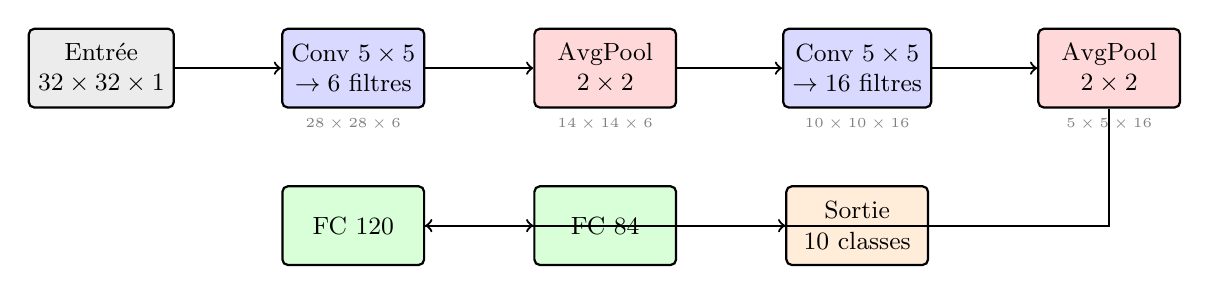
\begin{tikzpicture}[
  block/.style={rectangle, draw, thick, fill=#1, minimum height=1cm,
                minimum width=1.8cm, font=\small, align=center, rounded corners=2pt},
  block/.default={blue!15},
  arr/.style={->, thick}
]
  \node[block=gray!15] (input) at (0,0) {Entr\'ee\\$32 \times 32 \times 1$};
  \node[block] (c1) at (3.2,0) {Conv $5 \times 5$\\$\to 6$ filtres};
  \node[block=red!15] (p1) at (6.4,0) {AvgPool\\$2 \times 2$};
  \node[block] (c2) at (9.6,0) {Conv $5 \times 5$\\$\to 16$ filtres};
  \node[block=red!15] (p2) at (12.8,0) {AvgPool\\$2 \times 2$};
  \node[block=green!15] (fc1) at (3.2,-2) {FC 120};
  \node[block=green!15] (fc2) at (6.4,-2) {FC 84};
  \node[block=orange!15] (out) at (9.6,-2) {Sortie\\10 classes};

  \draw[arr] (input) -- (c1);
  \draw[arr] (c1) -- (p1);
  \draw[arr] (p1) -- (c2);
  \draw[arr] (c2) -- (p2);
  \draw[arr] (p2) |- (fc1);
  \draw[arr] (fc1) -- (fc2);
  \draw[arr] (fc2) -- (out);

  % Tailles
  \node[below, font=\tiny, gray] at (c1.south) {$28 \times 28 \times 6$};
  \node[below, font=\tiny, gray] at (p1.south) {$14 \times 14 \times 6$};
  \node[below, font=\tiny, gray] at (c2.south) {$10 \times 10 \times 16$};
  \node[below, font=\tiny, gray] at (p2.south) {$5 \times 5 \times 16$};
\end{tikzpicture}
\end{center}

\subsection{AlexNet (2012)}
\index{AlexNet}

AlexNet \cite{krizhevsky2012imagenet} a marqu\'e le retour des r\'eseaux de
neurones en vision par ordinateur, remportant le d\'efi ImageNet 2012 avec
une erreur top-5 de 15.3\% (contre 26.2\% pour les m\'ethodes classiques).
Innovations cl\'es : ReLU, Dropout (cf.\ chapitre~\ref{ch:regularisation}),
entra\^inement sur GPU.

\subsection{VGGNet (2014)}
\index{VGGNet}

VGGNet \cite{simonyan2015very} a d\'emontr\'e l'importance de la profondeur
avec une architecture homog\`ene utilisant uniquement des convolutions $3 \times 3$.

\begin{remarque}[Champ r\'eceptif de convolutions empil\'ees]
Deux convolutions $3 \times 3$ empil\'ees ont un champ r\'eceptif de $5 \times 5$,
et trois convolutions $3 \times 3$ ont un champ de $7 \times 7$, mais avec
moins de param\`etres : $3 \times (3^2 C^2) = 27C^2$ vs $7^2 C^2 = 49C^2$.
\end{remarque}

\subsection{ResNet (2015)}
\label{sec:resnet}
\index{ResNet}

\subsubsection{Connexion r\'esiduelle}

\begin{formules}[title=\textbf{Bloc r\'esiduel}]
\begin{equation}
\mathbf{y} = \mathcal{F}(\mathbf{x}, \{W_i\}) + \mathbf{x}
\label{eq:residual-block}
\end{equation}
o\`u $\mathcal{F}(\mathbf{x}, \{W_i\})$ repr\'esente la transformation
r\'esiduelle (typiquement Conv-BN-ReLU-Conv-BN).
\end{formules}

\begin{center}
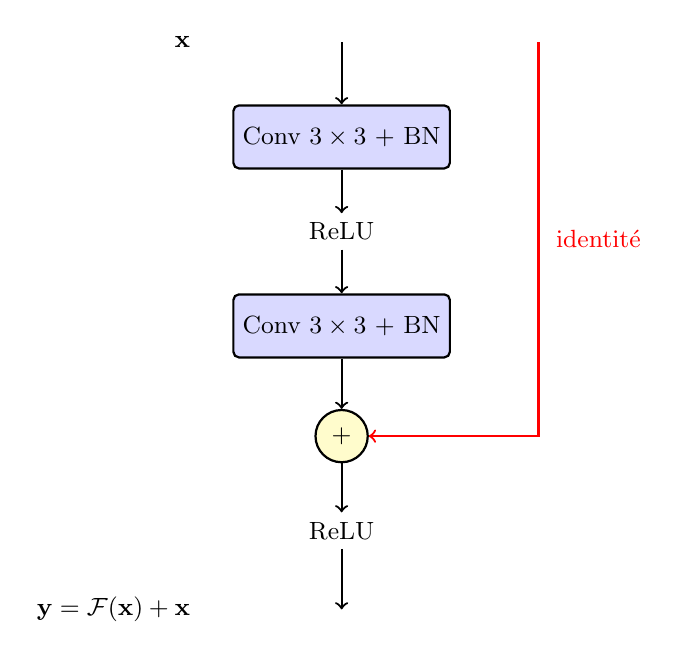
\begin{tikzpicture}[
  block/.style={rectangle, draw, thick, fill=blue!15, minimum height=0.8cm,
                minimum width=2.5cm, font=\small, rounded corners=2pt},
  arr/.style={->, thick},
  plus/.style={circle, draw, thick, fill=yellow!20, minimum size=6mm,
               font=\small}
]
  \node[block] (conv1) at (0, 0) {Conv $3 \times 3$ + BN};
  \node[font=\small] (relu1) at (0, -1.2) {ReLU};
  \node[block] (conv2) at (0, -2.4) {Conv $3 \times 3$ + BN};
  \node[plus] (add) at (0, -3.8) {$+$};
  \node[font=\small] (relu2) at (0, -5.0) {ReLU};

  % Connexion principale
  \draw[arr] (0, 1.2) -- (conv1);
  \draw[arr] (conv1) -- (relu1);
  \draw[arr] (relu1) -- (conv2);
  \draw[arr] (conv2) -- (add);
  \draw[arr] (add) -- (relu2);
  \draw[arr] (relu2) -- (0, -6.0);

  % Skip connection
  \draw[arr, red, thick] (2.5, 1.2) -- (2.5, -3.8) -- (add);
  \node[red, font=\small, right] at (2.6, -1.3) {identit\'e};

  % Labels
  \node[left, font=\small] at (-1.8, 1.2) {$\mathbf{x}$};
  \node[left, font=\small] at (-1.8, -6.0) {$\mathbf{y} = \mathcal{F}(\mathbf{x}) + \mathbf{x}$};
\end{tikzpicture}
\end{center}

\subsubsection{Preuve de la pr\'eservation du flux de gradient}

\begin{theoreme}[Flux de gradient dans ResNet]
\label{thm:resnet-gradient}
Soit un r\'eseau de $L$ blocs r\'esiduels. La sortie du bloc $l$ est
$\mathbf{x}_{l+1} = \mathcal{F}_l(\mathbf{x}_l) + \mathbf{x}_l$. Alors
la sortie du bloc $L$ peut s'exprimer comme :
\begin{equation}
\mathbf{x}_L = \mathbf{x}_l + \sum_{i=l}^{L-1} \mathcal{F}_i(\mathbf{x}_i)
\label{eq:resnet-unrolled}
\end{equation}

Le gradient de la perte $\mathcal{L}$ par rapport \`a $\mathbf{x}_l$ est :
\begin{align}
\frac{\partial \mathcal{L}}{\partial \mathbf{x}_l}
&= \frac{\partial \mathcal{L}}{\partial \mathbf{x}_L}
   \cdot \frac{\partial \mathbf{x}_L}{\partial \mathbf{x}_l} \nonumber \\
&= \frac{\partial \mathcal{L}}{\partial \mathbf{x}_L}
   \left(1 + \frac{\partial}{\partial \mathbf{x}_l}
   \sum_{i=l}^{L-1} \mathcal{F}_i(\mathbf{x}_i)\right)
\label{eq:resnet-gradient}
\end{align}

\textbf{D\'emonstration.}
Par r\'ecurrence, $\mathbf{x}_{l+1} = \mathcal{F}_l(\mathbf{x}_l) + \mathbf{x}_l$
et $\mathbf{x}_{l+2} = \mathcal{F}_{l+1}(\mathbf{x}_{l+1}) + \mathbf{x}_{l+1}
= \mathcal{F}_{l+1}(\mathbf{x}_{l+1}) + \mathcal{F}_l(\mathbf{x}_l) + \mathbf{x}_l$.
Par induction, on obtient (\ref{eq:resnet-unrolled}). En d\'erivant et en
appliquant la r\`egle de la cha\^ine, le terme $\mathbf{1}$ dans
(\ref{eq:resnet-gradient}) garantit que le gradient ne s'annule jamais
compl\`etement, m\^eme si $\frac{\partial \mathcal{F}_i}{\partial \mathbf{x}_l}
\to 0$.
\end{theoreme}

\begin{intuition}[title=\textbf{Pourquoi ResNet fonctionne}]
Le terme <<~$+1$~>> dans l'\'equation~(\ref{eq:resnet-gradient}) cr\'ee un
<<~autoroute \`a gradient~>> (gradient highway) qui contourne les couches
non lin\'eaires. Le r\'eseau n'a besoin d'apprendre que le \textbf{r\'esidu}
$\mathcal{F}(\mathbf{x}) = \mathbf{y} - \mathbf{x}$, qui est souvent proche
de z\'ero et donc plus facile \`a apprendre.
\end{intuition}

% ----------------------------------------------------------------------------
\section{Transfert d'apprentissage et fine-tuning}
\label{sec:transfer-learning}
\index{transfert d'apprentissage}\index{fine-tuning}

\begin{definition}[Transfert d'apprentissage]
Le transfert d'apprentissage consiste \`a r\'eutiliser un mod\`ele
pr\'e-entra\^in\'e sur un grand jeu de donn\'ees (ex.\ ImageNet) pour une
nouvelle t\^ache, \'eventuellement avec un jeu de donn\'ees plus petit.
\end{definition}

Strat\'egies courantes :
\begin{enumerate}
  \item \textbf{Extracteur de caract\'eristiques} : geler toutes les couches
    convolutives et n'entra\^iner que le classifieur final.
  \item \textbf{Fine-tuning partiel} : d\'egeler les derni\`eres couches
    convolutives avec un taux d'apprentissage r\'eduit.
  \item \textbf{Fine-tuning complet} : entra\^iner tout le r\'eseau avec un
    taux d'apprentissage faible.
\end{enumerate}

\begin{bonnepratique}[title=\textbf{Taux d'apprentissage pour le fine-tuning}]
Utiliser un taux d'apprentissage 10 \`a 100 fois plus petit que pour
l'entra\^inement initial. Les techniques de
r\'egularisation (chapitre~\ref{ch:regularisation}) sont cruciales pour
\'eviter le surapprentissage lors du fine-tuning.
\end{bonnepratique}

% ----------------------------------------------------------------------------
\section{Impl\'ementation PyTorch}
\label{sec:cnn-pytorch}

\begin{codeblock}[title=\textbf{CNN pour CIFAR-10 avec entra\^inement complet}]
\begin{minted}{python}
import torch
import torch.nn as nn
import torch.optim as optim
from torchvision import datasets, transforms
from torch.utils.data import DataLoader

# --- Architecture CNN ---
class CIFAR10Net(nn.Module):
    def __init__(self, num_classes=10):
        super().__init__()
        self.features = nn.Sequential(
            # Bloc 1: 32x32x3 -> 32x32x64 -> 16x16x64
            nn.Conv2d(3, 64, kernel_size=3, padding=1),
            nn.BatchNorm2d(64),
            nn.ReLU(inplace=True),
            nn.Conv2d(64, 64, kernel_size=3, padding=1),
            nn.BatchNorm2d(64),
            nn.ReLU(inplace=True),
            nn.MaxPool2d(2, 2),
            nn.Dropout2d(0.25),

            # Bloc 2: 16x16x64 -> 16x16x128 -> 8x8x128
            nn.Conv2d(64, 128, kernel_size=3, padding=1),
            nn.BatchNorm2d(128),
            nn.ReLU(inplace=True),
            nn.Conv2d(128, 128, kernel_size=3, padding=1),
            nn.BatchNorm2d(128),
            nn.ReLU(inplace=True),
            nn.MaxPool2d(2, 2),
            nn.Dropout2d(0.25),

            # Bloc 3: 8x8x128 -> 8x8x256 -> 4x4x256
            nn.Conv2d(128, 256, kernel_size=3, padding=1),
            nn.BatchNorm2d(256),
            nn.ReLU(inplace=True),
            nn.Conv2d(256, 256, kernel_size=3, padding=1),
            nn.BatchNorm2d(256),
            nn.ReLU(inplace=True),
            nn.MaxPool2d(2, 2),
            nn.Dropout2d(0.25),
        )
        self.classifier = nn.Sequential(
            nn.AdaptiveAvgPool2d(1),   # Global Average Pooling
            nn.Flatten(),
            nn.Linear(256, 128),
            nn.ReLU(inplace=True),
            nn.Dropout(0.5),
            nn.Linear(128, num_classes)
        )

    def forward(self, x):
        x = self.features(x)
        x = self.classifier(x)
        return x

# --- Pr'eparation des donn'ees ---
transform_train = transforms.Compose([
    transforms.RandomCrop(32, padding=4),
    transforms.RandomHorizontalFlip(),
    transforms.ColorJitter(brightness=0.2, contrast=0.2),
    transforms.ToTensor(),
    transforms.Normalize((0.4914, 0.4822, 0.4465),
                         (0.2470, 0.2435, 0.2616))
])

transform_test = transforms.Compose([
    transforms.ToTensor(),
    transforms.Normalize((0.4914, 0.4822, 0.4465),
                         (0.2470, 0.2435, 0.2616))
])

train_set = datasets.CIFAR10('./data', train=True,
                             download=True, transform=transform_train)
test_set = datasets.CIFAR10('./data', train=False,
                            transform=transform_test)
train_loader = DataLoader(train_set, batch_size=128,
                          shuffle=True, num_workers=2)
test_loader = DataLoader(test_set, batch_size=256,
                         shuffle=False, num_workers=2)

# --- Entra^inement ---
device = torch.device('cuda' if torch.cuda.is_available() else 'cpu')
model = CIFAR10Net().to(device)
criterion = nn.CrossEntropyLoss()
optimizer = optim.AdamW(model.parameters(), lr=1e-3, weight_decay=1e-4)
scheduler = optim.lr_scheduler.CosineAnnealingLR(optimizer, T_max=100)

print(f"Param`etres: {sum(p.numel() for p in model.parameters()):,}")

for epoch in range(100):
    # Entra^inement
    model.train()
    train_loss, correct, total = 0.0, 0, 0
    for inputs, targets in train_loader:
        inputs, targets = inputs.to(device), targets.to(device)
        optimizer.zero_grad()
        outputs = model(inputs)
        loss = criterion(outputs, targets)
        loss.backward()
        optimizer.step()
        train_loss += loss.item() * inputs.size(0)
        correct += (outputs.argmax(1) == targets).sum().item()
        total += targets.size(0)

    # 'Evaluation
    model.eval()
    test_correct, test_total = 0, 0
    with torch.no_grad():
        for inputs, targets in test_loader:
            inputs, targets = inputs.to(device), targets.to(device)
            outputs = model(inputs)
            test_correct += (outputs.argmax(1) == targets).sum().item()
            test_total += targets.size(0)

    scheduler.step()
    if (epoch + 1) % 10 == 0:
        print(f"Epoch {epoch+1:3d} | "
              f"Train Loss: {train_loss/total:.4f} | "
              f"Train Acc: {correct/total:.4f} | "
              f"Test Acc: {test_correct/test_total:.4f}")
\end{minted}
\end{codeblock}

\begin{codeoutput}
\begin{verbatim}
Param`etres: 952,202
Epoch  10 | Train Loss: 0.8234 | Train Acc: 0.7142 | Test Acc: 0.7856
Epoch  20 | Train Loss: 0.5321 | Train Acc: 0.8134 | Test Acc: 0.8523
Epoch  30 | Train Loss: 0.4012 | Train Acc: 0.8612 | Test Acc: 0.8802
Epoch  40 | Train Loss: 0.3245 | Train Acc: 0.8876 | Test Acc: 0.8945
Epoch  50 | Train Loss: 0.2678 | Train Acc: 0.9056 | Test Acc: 0.9034
Epoch  60 | Train Loss: 0.2234 | Train Acc: 0.9213 | Test Acc: 0.9098
Epoch  70 | Train Loss: 0.1878 | Train Acc: 0.9345 | Test Acc: 0.9145
Epoch  80 | Train Loss: 0.1534 | Train Acc: 0.9467 | Test Acc: 0.9178
Epoch  90 | Train Loss: 0.1312 | Train Acc: 0.9534 | Test Acc: 0.9201
Epoch 100 | Train Loss: 0.1198 | Train Acc: 0.9578 | Test Acc: 0.9218
\end{verbatim}
\end{codeoutput}

% ----------------------------------------------------------------------------
\section{Transfer learning avec un mod\`ele pr\'e-entra\^in\'e}
\label{sec:transfer-code}

\begin{codeblock}[title=\textbf{Fine-tuning d'un ResNet-18 pr\'e-entra\^in\'e}]
\begin{minted}{python}
import torchvision.models as models

# Charger ResNet-18 pr'e-entra^in'e sur ImageNet
model = models.resnet18(weights=models.ResNet18_Weights.DEFAULT)

# Geler les couches convolutives
for param in model.parameters():
    param.requires_grad = False

# Remplacer la derni`ere couche FC
num_features = model.fc.in_features
model.fc = nn.Sequential(
    nn.Dropout(0.3),
    nn.Linear(num_features, 10)
)
model = model.to(device)

# Seule la derni`ere couche est entra^in'ee
optimizer = optim.Adam(model.fc.parameters(), lr=1e-3)

# Phase 2 : d'egeler les 2 derniers blocs pour fine-tuning
for param in model.layer3.parameters():
    param.requires_grad = True
for param in model.layer4.parameters():
    param.requires_grad = True

optimizer = optim.AdamW([
    {'params': model.layer3.parameters(), 'lr': 1e-5},
    {'params': model.layer4.parameters(), 'lr': 1e-4},
    {'params': model.fc.parameters(), 'lr': 1e-3},
], weight_decay=1e-4)
\end{minted}
\end{codeblock}

% ----------------------------------------------------------------------------
\section{\'Etude d'ablation}
\label{sec:cnn-ablation}

\begin{codeblock}[title=\textbf{Ablation : taille du noyau, nombre de filtres, profondeur}]
\begin{minted}{python}
import pandas as pd

def build_cnn(kernel_size, num_filters, num_blocks):
    """Construit un CNN param'etrable pour l'ablation."""
    layers = []
    in_channels = 3
    for i in range(num_blocks):
        out_channels = num_filters * (2 ** min(i, 2))
        pad = kernel_size // 2
        layers.extend([
            nn.Conv2d(in_channels, out_channels, kernel_size, padding=pad),
            nn.BatchNorm2d(out_channels),
            nn.ReLU(inplace=True),
            nn.MaxPool2d(2, 2),
        ])
        in_channels = out_channels
    layers.extend([nn.AdaptiveAvgPool2d(1), nn.Flatten(),
                   nn.Linear(in_channels, 10)])
    return nn.Sequential(*layers)

configs = [
    {'kernel_size': 3, 'num_filters': 32, 'num_blocks': 3},
    {'kernel_size': 5, 'num_filters': 32, 'num_blocks': 3},
    {'kernel_size': 3, 'num_filters': 64, 'num_blocks': 3},
    {'kernel_size': 3, 'num_filters': 32, 'num_blocks': 5},
]

results = []
for cfg in configs:
    model = build_cnn(**cfg).to(device)
    n_params = sum(p.numel() for p in model.parameters())
    # Entra^iner 30 'epoques (simplifi'e)
    optimizer = optim.AdamW(model.parameters(), lr=1e-3)
    best_acc = 0.0
    for epoch in range(30):
        model.train()
        for x, y in train_loader:
            x, y = x.to(device), y.to(device)
            optimizer.zero_grad()
            loss = criterion(model(x), y)
            loss.backward()
            optimizer.step()
        model.eval()
        correct = sum((model(x.to(device)).argmax(1) == y.to(device)).sum().item()
                      for x, y in test_loader)
        best_acc = max(best_acc, correct / len(test_set))
    results.append({**cfg, 'params': n_params, 'accuracy': best_acc})

print(pd.DataFrame(results).to_string(index=False))
\end{minted}
\end{codeblock}

\begin{codeoutput}
\begin{verbatim}
 kernel_size  num_filters  num_blocks  params   accuracy
           3           32           3   52778     0.8734
           5           32           3  143642     0.8812
           3           64           3  207946     0.9015
           3           32           5  218410     0.8956
\end{verbatim}
\end{codeoutput}

\begin{remarque}[Observations de l'ablation]
\begin{itemize}
  \item Doubler le nombre de filtres ($32 \to 64$) am\'eliore davantage les
    performances que d'augmenter la taille du noyau ou la profondeur.
  \item Les noyaux $5 \times 5$ apportent un gain marginal par rapport aux
    $3 \times 3$ pour un co\^ut en param\`etres significatif.
  \item La profondeur aide, mais avec des rendements d\'ecroissants sans
    connexions r\'esiduelles.
\end{itemize}
\end{remarque}

% ----------------------------------------------------------------------------
\section{Convolutions s\'eparables en profondeur}
\label{sec:depthwise-separable}
\index{convolution!s\'eparable en profondeur}

\begin{formules}[title=\textbf{Convolution s\'eparable en profondeur}]
Une convolution standard $C_{\text{in}} \to C_{\text{out}}$ avec noyau $k \times k$
co\^ute $C_{\text{in}} \cdot C_{\text{out}} \cdot k^2$ multiplications par position.
La convolution s\'eparable d\'ecompose en :
\begin{enumerate}
  \item \textbf{Depthwise} : un filtre $k \times k$ par canal, co\^ut $C_{\text{in}} \cdot k^2$
  \item \textbf{Pointwise} : convolution $1 \times 1$ pour combiner, co\^ut $C_{\text{in}} \cdot C_{\text{out}}$
\end{enumerate}
Ratio de r\'eduction :
\begin{equation}
\frac{C_{\text{in}} \cdot k^2 + C_{\text{in}} \cdot C_{\text{out}}}{C_{\text{in}} \cdot C_{\text{out}} \cdot k^2}
= \frac{1}{C_{\text{out}}} + \frac{1}{k^2}
\end{equation}
Pour $C_{\text{out}} = 256$ et $k = 3$ : r\'eduction d'un facteur $\approx 8\text{--}9\times$.
\end{formules}

% ----------------------------------------------------------------------------
\section{Techniques \'etat de l'art}
\label{sec:cnn-sota}

\begin{sota}[title=\textbf{Architectures CNN modernes}]
\begin{description}
  \item[EfficientNet] \cite{tan2019efficientnet} : mise \`a l'\'echelle
    compos\'ee \'equilibr\'ee en profondeur, largeur et r\'esolution :
    \begin{equation}
      d = \alpha^\phi, \quad w = \beta^\phi, \quad r = \gamma^\phi
      \quad \text{sous} \quad \alpha \cdot \beta^2 \cdot \gamma^2 \approx 2
    \end{equation}
    \index{EfficientNet}

  \item[ConvNeXt] \cite{liu2022convnet} : modernisation de ResNet avec des
    \'el\'ements emprunt\'es aux Transformers (cf.\ chapitre~\ref{ch:attention}) :
    noyaux $7 \times 7$ depthwise, LayerNorm, GELU, fewer activation functions.
    Atteint des performances comparables aux Vision Transformers.
    \index{ConvNeXt}

  \item[Convolutions d\'eformables] \cite{dai2017deformable} : apprennent des
    offsets spatiaux pour adapter la forme du champ r\'eceptif :
    \begin{equation}
      y(\mathbf{p}_0) = \sum_{n=1}^{N} w_n \cdot x(\mathbf{p}_0 + \mathbf{p}_n + \Delta\mathbf{p}_n)
    \end{equation}
    o\`u $\Delta\mathbf{p}_n$ sont des offsets appris.
    \index{convolution!d\'eformable}
\end{description}
\end{sota}

% ----------------------------------------------------------------------------
\section{Exercices}
\label{sec:cnn-exercices}

\begin{exercice}[Calculs de dimensions \hfill $\bigstar$]
Un r\'eseau re\c{c}oit des images $128 \times 128 \times 3$ et applique
successivement :
\begin{enumerate}
  \item Conv2d(3, 32, kernel\_size=5, padding=2, stride=1)
  \item MaxPool2d(2, 2)
  \item Conv2d(32, 64, kernel\_size=3, padding=0, stride=2)
  \item Conv2d(64, 128, kernel\_size=3, padding=1, stride=1)
  \item AdaptiveAvgPool2d(1)
\end{enumerate}
Calculer la taille de sortie et le nombre de param\`etres \`a chaque couche.
\end{exercice}

\begin{exercice}[Impl\'ementation d'un bloc r\'esiduel \hfill $\bigstar\bigstar$]
\begin{enumerate}
  \item Impl\'ementer un bloc r\'esiduel complet (avec projection si les
    dimensions changent) en PyTorch.
  \item Construire un mini-ResNet (8 couches) pour CIFAR-10.
  \item Comparer la convergence avec et sans connexions r\'esiduelles.
  \item Tracer les gradients dans les premi\`eres couches pour les deux cas.
\end{enumerate}
\end{exercice}

\begin{exercice}[Visualisation des filtres \hfill $\bigstar\bigstar$]
\begin{enumerate}
  \item Entra\^iner un CNN sur CIFAR-10 et visualiser les filtres de la
    premi\`ere couche convolutive.
  \item Utiliser les \textit{feature maps} interm\'ediaires pour comprendre
    ce que chaque couche d\'etecte.
  \item Impl\'ementer la technique de \textit{Grad-CAM} pour visualiser les
    r\'egions de l'image contribuant \`a la d\'ecision.
\end{enumerate}
\end{exercice}

\begin{exercice}[Convolutions s\'eparables en profondeur \hfill $\bigstar\bigstar$]
\begin{enumerate}
  \item Impl\'ementer une couche de convolution s\'eparable en profondeur
    (\texttt{nn.Conv2d} avec \texttt{groups=in\_channels} + conv $1 \times 1$).
  \item Remplacer toutes les convolutions $3 \times 3$ du CNN CIFAR-10 par
    des convolutions s\'eparables. Comparer le nombre de param\`etres et la
    pr\'ecision.
  \item Mesurer le temps d'inf\'erence des deux versions.
\end{enumerate}
\end{exercice}

\begin{exercice}[Preuve du champ r\'eceptif \hfill $\bigstar\bigstar\bigstar$]
\begin{enumerate}
  \item D\'emontrer par r\'ecurrence que $n$ couches convolutives $k \times k$
    empil\'ees avec stride $s = 1$ produisent un champ r\'eceptif de taille
    $n(k - 1) + 1$.
  \item G\'en\'eraliser pour des strides et dilations arbitraires.
  \item Calculer le champ r\'eceptif effectif d'un ResNet-50 et comparer avec
    la taille de l'image d'entr\'ee.
  \item Discuter le lien entre champ r\'eceptif et capacit\'e de
    mod\'elisation.
\end{enumerate}
\end{exercice}
